\documentclass{beamer}
\usetheme{metropolis}

\usepackage{xcolor}
\usepackage{graphicx}
\usepackage{tcolorbox}
\usepackage{listings}
\usepackage{booktabs}
\usepackage{array}
\usepackage{tabularx}
\usepackage{lmodern}
\usefonttheme[onlymath]{serif}

\begin{document}
\newcommand{\tabitem}{~~\llap{\textbullet}~~}

\definecolor{codegreen}{rgb}{0,0.6,0}
\definecolor{codegray}{rgb}{0.5,0.5,0.5}
\definecolor{codepurple}{rgb}{0.58,0,0.82}
\definecolor{backcolour}{rgb}{0.95,0.95,0.92}

\lstset{
	language=C++,
	basicstyle=\scriptsize\ttfamily,
	keywordstyle=\color{magenta},
	stringstyle=\color{codepurple},
	numbers=left,
	numbersep=5pt,
	numberstyle=\tiny\color{codegray},
	backgroundcolor=\color{backcolour},
	showstringspaces=false,
	tabsize=4
}


\title{Asymptotic Analysis}
\subtitle{Think Big}
\author{UTEC - Competitive Programming}
\date{}

\maketitle

\begin{frame}
	\frametitle{Complexity}

	\begin{itemize}
		\item When describing the performance of an algorithm, the word complexity is commonly used.
		\item Complexity can be considered as the amount of resources my algorithm will consume:
			\begin{itemize}
				\item \textbf{Time Complexity:} How long will my program take to run for a given input.
				\item \textbf{Space Complexity:} How much memory will my program consume for a given input.
			\end{itemize}
		\item In many cases there exists a trade-off between space and time complexity. More memory = Less time
	\end{itemize}
\end{frame}

\begin{frame}
	\frametitle{Challenge}

	Lets find a solution for the following problem:
	\begin{center}
		Given an array $a$ with $n$ elements, find the smallest one. $n \leq 10^6$
	\end{center}

	\begin{itemize}
		\item<2-> How long will your solution take if $n = 10^3, 10^5, 10^6$
		\item<3-> How many solutions there are to this problem?
		\item<4-> Is this solution the best solution?
		\item<5-> How can we compare solutions?
	\end{itemize}
\end{frame}


\section{Measuring Complexity}

\begin{frame}
	\frametitle{Sampling and Extrapolation}

	\begin{itemize}
		\item One first approach to measuring complexity can be to manually measure how long our solution takes to run for different inputs.
		\item We can then try to extrapolate our measurments and attempt to predict the time our program will take for other inputs.
		\item Let's try it out!
	\end{itemize}
\end{frame}

\begin{frame}
	\frametitle{Sampling and Extrapolation - Problems}

	\begin{itemize}
		\item Easy to miss \textbf{corner cases}.
		\item Takes a lot of time.
		\item Requires a lot of guessing.
		\item Sometimes it is really hard to generate input.
	\end{itemize}
\end{frame}

\begin{frame}
	\frametitle{Changing Perspective}
	
	\begin{itemize}
		\item Lets define the function $T(x)$ as the time our algorithm takes to run for an input $x$.
		\item Lets also define $N(x)$, as the number of instructions our algorithm takes for an input $x$.
		\item It is simple to see that $T(x) \alpha N(x)$
	\end{itemize}
\end{frame}

\begin{frame}
	\frametitle{Changing Perspective}
	
	\begin{itemize}
		\item Overall, we can say that:
			$$T(x) = kN(x)$$
		\item What would $k$ represent in this equation?
		\item $k_{C++} \approx 10^8$, $k_{py} \approx 10^6$
		\item Counting the number of steps is esay! ... \textit{usually}
	\end{itemize}
\end{frame}

\begin{frame}
	\frametitle{Counting instructions}

	\begin{itemize}
		\item The goal is to count how many basic instructions are executed during an algorithm.
		\item Assume that basic instructions are those that can be executed natively by the computer:
			\begin{itemize}
				\item addition, subtraction, multiplication, division, remainder
				\item modifying and calling variables
				\item calling functions
				\item etc...
			\end{itemize}
		\item We assume that all instructions take the same time.
		\item Find $N(n)$ for the following solutions
	\end{itemize}
\end{frame}

\begin{frame}[fragile]
	\frametitle{Counting instructions - Practice}
	\lstinputlisting{listings/min1.cpp}
\end{frame}

\begin{frame}[fragile]
	\frametitle{Counting instructions - Practice}
	\lstinputlisting{listings/min2.cpp}
\end{frame}


\section{Asymptotic Analysis}

\begin{frame}
	\frametitle{Asymptotic Analysis - Introduction}

	\begin{itemize}
		\item It is a method for defining the mathemathical boundry of the run-time performance of an algorithm.
		\item Using asymptotic analysis we look to find:
			\begin{itemize}
				\item Lower Bound - $\Omega(f(n))$ Big Omega Notation
				\item Tight Bound - $\Theta(f(n))$ Big Theta Notation
				\item \textbf{Upper Bound - $O(f(n))$ Big Oh Notation}
			\end{itemize}
		\item In competitive programming we only care about $O(n)$. \textbf{Why?}
	\end{itemize}
\end{frame}

\begin{frame}
	\frametitle{Big Oh - A Formal Introduction}

	\begin{itemize}
		\item $O(f(n))$ is a set that contains all functions that are asymptotically smaller than $f(n)$.
		\item Formally:
			$$f(n) = O(g(n)) \rightarrow f(n) < kg(n)$$ 
			For $n > n_0$, $n_0 \in \mathbb{N}$ and $ k > 0$
	\end{itemize}

	\begin{center}
		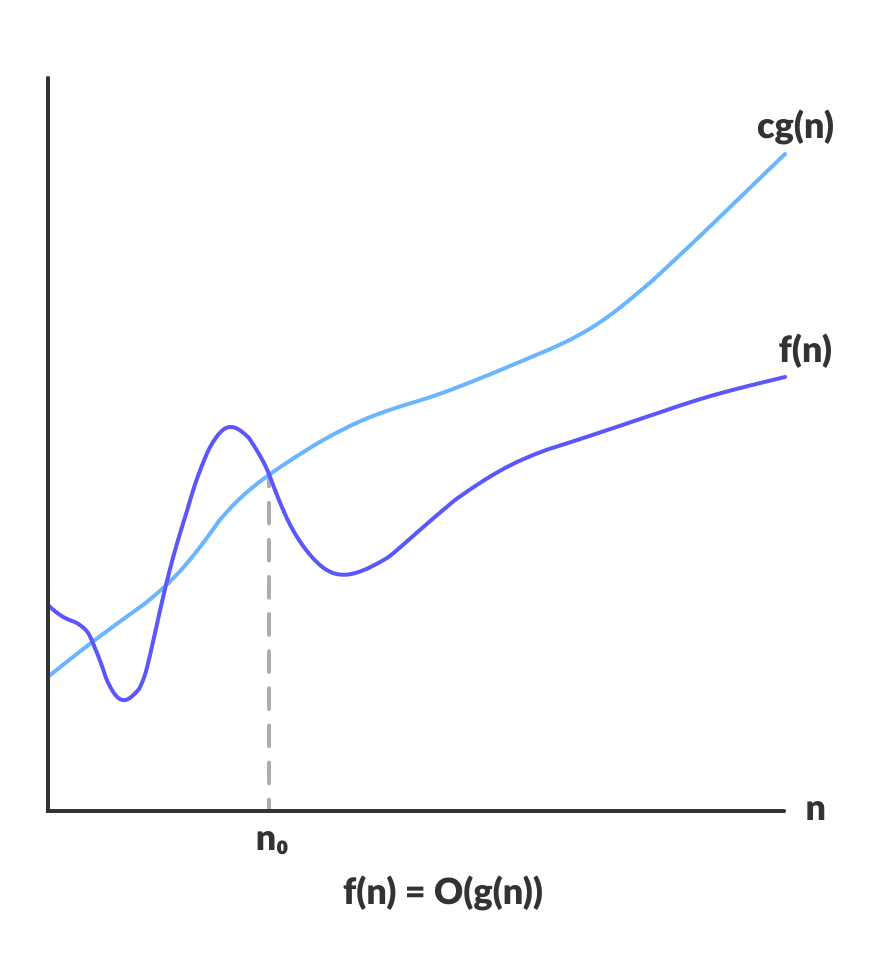
\includegraphics[scale=0.25]{images/big-oh}
	\end{center}
\end{frame}

\begin{frame}
	\frametitle{Big Oh - In Practice}

	\begin{itemize}
		\item In general lets say we can estimate that our program has a time complexity of:
			$$T(n) = a_mn^m a_{m - 1}n^{m - 1} + \ldots + a_1n + a_0$$
		\item It is simple to see that as $n$ gets bigger, $T(n)$ will be more heavily dominated by its largest term.
		\item Therefore,$T(n) \approx n^m$, for sufficiently large $n$.
		\item We can also realize that $T(n) = O(n^m)$. \textbf{Why?}
		\item Now that we know we only care about the largest term calculating $T(n)$ should be much faster!
	\end{itemize}
\end{frame}

\begin{frame}
	\frametitle{Using Asymptotic Analysis}

	In general, from the constrains of a problem we can get the expected complexity our solution should have. For example:

	\begin{table}[]
		\bgroup
		\setlength\tabcolsep{10pt}.
		\begin{tabular}{l|c}
			\multicolumn{1}{c|}{\textbf{Input Size}} & \multicolumn{1}{c}{\textbf{Maximum Valid Complexity}} \\ \hline
			$n \leq 10$ & $O(n!)$ \\
			$n \leq 20$ & $O(2^n)$ \\
			$n \leq 500$ & $O(n^3)$ \\
			$n \leq 5000$ & $O(n^2)$ \\
			$n \leq 10^6$ & $O(nlgn)$ \\
			$n \leq 10^7$ & $O(n)$ \\
			$n > 10^7$ & $O(1)$ or $O(lgn)$
		\end{tabular}
		\egroup
	\end{table}
\end{frame}

\end{document}
